\documentclass[10pt,twocolumn]{article}
\usepackage[a4paper,margin=0.8in,columnsep=0.25in]{geometry}
\usepackage[T1]{fontenc}
\usepackage{lmodern,microtype,booktabs,graphicx,amsmath,hyperref,caption,array}
\usepackage[numbers,sort&compress]{natbib}
\captionsetup{font=small,labelfont=bf}
\hypersetup{colorlinks=true,linkcolor=black,citecolor=black,urlcolor=blue}
\setlength{\parskip}{2pt}
\newcommand{\dP}{\Delta P}

\title{Which Stem Carries the Era of a Song, and Can a Generator Be Steered to It?\\
\large Stem-wise probes of release decade and release market, and era-targeted accompaniment regeneration on Discogs-VI clips}
\author{James Christian\\ {\small University of Texas at Austin}\\ {\small\texttt{jameschristian@utexas.edu}}
\and Liang-Yu Hsia\\ {\small National Taiwan University (GICE)}\\ {\small\texttt{r13942129@ntu.edu.tw}}
\and Jefferson Sy Dionisio\\ {\small National Taiwan University (GICE)}\\ {\small\texttt{jsydionisio@gmail.com}}}
\date{}

\begin{document}
\maketitle

\begin{abstract}
We ask two connected questions on a subset of Discogs-VI clips: which part of a recording (vocal stem, accompaniment stem, or the mix) lets frozen audio encoders recognise the release \emph{decade} and the release \emph{market}, and can a generator that keeps the original vocal and melody regenerate the accompaniment in a requested decade. With linear probes, stem recombination, concept erasure and signal-level controls we find that decade information is carried by the accompaniment at least as much as by the vocal, whereas market information follows the vocal stem and is largely, but not entirely, explained by sung language. For generation we keep the original vocal, condition MusicGen-Melody on the chroma of the original mix, fine-tune a low-rank adapter on decade-labelled accompaniment and add a three-branch guidance rule that keeps the melody term and adds an era-contrast term. With codec-matched probes of two encoders, an independent third encoder, and distribution and pairing metrics, the system orders six prompted decades monotonically in expected decade and largely keeps song identity (chroma song-identification top-1 $0.875$ against $0.944$ for neutral generations of the same adapter), while the unmodified model moves only the 1980s and 2010s. We also report where the evidence is weak: probes respond to bandwidth cues, the 1990s prompt is wording-dependent, and no listening test was run.
\end{abstract}

\section{Introduction}
Release decade and release market are weak, edition-level labels: in the full Discogs-VI metadata a composition has on average $2.42$ distinct release countries and $1.99$ distinct release decades (Sec.~\ref{sec:data}). Still, models trained on them are used as ``era'' or ``region'' detectors, and generators are asked to produce music ``in the style of the 1980s''. Two questions follow. (i) Which \emph{part} of a recording, and which \emph{cue} (sung language, genre, recording bandwidth), does a detector actually use? (ii) If a stable cue exists, can it be used to steer a cover that keeps the original melody and vocal?

Related work is reviewed in Sec.~\ref{sec:rel}. This is mainly an empirical study: the adapter and the guidance rule combine existing techniques, and we claim no new architecture.

\textbf{Contributions.} (1) A stem-wise analysis with causal-style interventions (stem swap, linear erasure with random-rank controls, retrained-probe cue ablations) on two tasks. (2) An era-controllable cover system built from a public generator, an adapter and a guidance rule, evaluated with codec-matched probes, an independent encoder, a zero-shot audio-language judge, distribution and pairing metrics, and content-preservation metrics. (3) Controls that show what the probes also respond to (bandwidth, spectral balance, wording), reported with the main result rather than separately.

\section{Related work}\label{sec:rel}
\textbf{Era recognition.} Year prediction from audio was introduced as the showcase task of the Million Song Dataset~\cite{bertin2011msd}; He et al.~\cite{he2024era} frame era recognition as classification into year ranges with supervised contrastive learning and artist information; Lee et al.~\cite{lee2026era} classify the first-entry era of US and Korean pop from audio and name as their main limitation that models cannot separate compositional style from recording technology. None of these separates stems or tests which cue a detector uses by intervention, which our analysis does; none uses release era as a control signal for generation.

\textbf{Cues and confounds.} Hsieh et al.~\cite{hsieh2020confounds} remix vocals with accompaniments of other songs to study confounds in singer identification; we use the same intervention. LEACE~\cite{belrose2023leace} gives a closed-form linear eraser, which we use with random-rank controls.

\textbf{Controllable and melody-preserving generation.} MusicGen-Melody~\cite{copet2023musicgen} conditions on chroma and text, which is the mechanism we use. Music ControlNet~\cite{wu2023musiccontrolnet}, JASCO~\cite{tal2024jasco}, ControlNet for Stable Audio Open~\cite{hou2024editing} (top-$k$ CQT melody control, motivated by the ambiguity of chroma) and MuseControlLite~\cite{tsai2025musecontrollite} add time-varying melody, rhythm or dynamics control, and are stronger melody-control baselines than ours; we compare only with MuseControlLite (Sec.~\ref{sec:gen}). Our conditioning is full-mix chroma, which is not the vocal melody; we did not ablate richer representations.

\textbf{Covers.} SongEcho~\cite{songecho2026} conditions on the vocal melody and text and generates new vocals and accompaniment; Demerl\'e et al.~\cite{demerle2024style} transfer genre style while carrying over rhythm and melody. Both target style or text control, not a release-decade axis, and we did not evaluate their systems. To our knowledge we did not find prior work that evaluates release decade as a controlled attribute of a melody-preserving cover; this is the result of a search and not a proof of absence.

\textbf{Our delta.} Relative to MusicGen-Melody: (i) an adapter trained on decade-labelled accompaniment; (ii) a three-branch guidance rule that keeps the melody term and adds an era-contrast term; (iii) an evaluation of decade control with nuisance controls. The probes used to evaluate are proxies for era, not human judgments.

\section{Data and protocol}\label{sec:data}
\textbf{Clips.} We use 30\,s mono 24\,kHz excerpts from Discogs-VI recordings~\cite{araz2024discogsvi} with artist-disjoint splits. Dataset A (decade, six classes 1960s--2010s): 1026 train, 132 validation clips with labels. Dataset B (market: US, UK, Brazil, Spain, Germany, Italy; all released in the 1980s): 798 train, 102 validation. Test labels are hidden, so all accuracies are on the validation split (chance $.167$). The audio is YouTube-sourced and may not be redistributed; we release code and result tables, not audio.

\textbf{Stems.} HT Demucs~\cite{rouard2022htdemucs} separates vocals from drums+bass+other (accompaniment); BS-RoFormer is used as a second separator. Stems are loudness-normalised to $-23$\,LUFS.

\textbf{Probes.} Frozen MERT-v2-30s~\cite{li2023mert} and MuQ~\cite{zhu2025muq} hidden states, mean-pooled over time; standardised logistic regression, layer and $C$ chosen by cross-validation on train only, scored once on validation; 95\% bootstrap intervals over clips; exact McNemar tests with Holm correction. Single-split differences below about $.05$ are within layer-selection noise (a 3-fold choice gives mix $.523$ instead of $.477$ on A), and intervals span about $\pm.09$.

\textbf{Label semantics.} In the full Discogs-VI metadata ($1.91$\,M versions, $348{,}796$ cliques), $62.1\%$ of cliques have $\geq 2$ release countries and $60.0\%$ have $\geq 2$ release decades; $44.1\%$ of 1980s versions in the six market countries sit in a clique with a 1980s version in another of the six. A release-market or release-decade label is therefore a property of an edition, not necessarily of the recording: a 1978 recording reissued in 1992 can carry a 1990s label although no acoustic property changed. We therefore speak of \emph{release decade} and treat probe and steering results as statements about decade-correlated audio properties, not recording era. (Our clips carry no Discogs ids, so these statistics describe the full metadata, not our subset.)

\section{Which stem carries the cue}
\begin{table}[t]\centering\small
\caption{Validation accuracy of linear probes (A: $n{=}132$, B: $n{=}102$; chance $.167$).}\label{tab:stems}
\begin{tabular}{@{}llcccc@{}}\toprule
Task & Encoder & Mix & Vocals & Accomp. & Recomb.\\\midrule
A decade & MERT & .477 & .394 & .485 & .485\\
 & MuQ & .477 & .318 & .424 & --\\
B market & MERT & .588 & .608 & .422 & .608\\
 & MuQ & .471 & .471 & .392 & --\\\bottomrule
\end{tabular}
\end{table}

Table~\ref{tab:stems} shows the pattern: for decade the accompaniment is as informative as the mix, the vocal stem is lower; for market the vocal stem is as informative as the mix and the accompaniment is lower. After Holm correction, the significant contrasts are mix vs.\ vocals on A with MuQ (adjusted $p{=}.012$) and, on B with MERT, mix vs.\ accompaniment ($.038$) and vocals vs.\ accompaniment ($.022$); MERT vocals vs.\ accompaniment on A ($p{=}.073$ before correction) is not significant. Re-summing the separated stems reproduces the mix accuracy ($.485$, $.608$), so separation itself does not change the result. BS-RoFormer reproduces the ordering (MERT, A: vocals $.386$, accompaniment $.515$; B: $.549$ vs.\ $.392$), but vocal-stem probes lose $.08$--$.13$ accuracy when the separator at test time differs from the one at training time, so absolute stem accuracies depend on the separator. Richer probes (MLP, SVM, layer concatenation, stem or encoder fusion), other pooling statistics, a layer-weighted sum, and five encoders (MERT, MuQ, Whisper, AST, CLAP) do not change the ordering; MERT is best or tied on every condition. Accuracy has not saturated with training size for A.

\begin{table}[t]\centering\small
\caption{Interventions on what the probes use (MERT, validation).}\label{tab:interv}
\begin{tabular}{@{}p{3.1cm}p{4.2cm}@{}}\toprule
Intervention & Result\\\midrule
Shuffle-and-remix: vocal of clip $i$ + accompaniment of clip $j$, other label (A: 396 pairs, B: 306)
& A: prediction = accompaniment label $34.8\%$ [29.5, 39.9] vs.\ vocal label $16.4\%$ [12.1, 21.0]. B: vocal label $50.0\%$ [42.2, 58.2] vs.\ accompaniment label $18.3\%$ [13.1, 23.5]. Same with BS-RoFormer.\\
LEACE erasure of the language subspace (B, rank 5) & mix $.588\to.353$, vocals $.608\to.402$, accomp. $.422\to.314$; random same-rank erasure: $.591$, $.606$, $.413$. A (85\% English): no change.\\
English-sung clips only (B, pooled out-of-fold) & mix $.397$ (majority share $.274$) vs.\ $.591$ on all clips.\\
LEACE erasure of style PCs (Discogs-EffNet tags; $k{=}10$) & A mix $.477\to.409$ (random $.49$); B accomp.\ $.422\to.294$.\\\bottomrule
\end{tabular}
\end{table}

Table~\ref{tab:interv} separates cues. Swapping stems shows that the \emph{decade} label follows the accompaniment and the \emph{market} label follows the vocal (cluster bootstrap over vocal clips). Erasing the linear subspace of Whisper-LID language~\cite{radford2022whisper} groups, with a same-rank random control~\cite{belrose2023leace}, removes most of the market accuracy while random erasure costs nothing; the result is unchanged when the language groups come from Whisper-large-v3 instead of Whisper-small ($.382$, $.392$, $.314$). Language labels are a proxy (no ground truth exists for these clips; the two LID models agree on $87.6\%$ of B clips after grouping). For decade, erasing style directions lowers accuracy more than random erasure, so part of the decade signal is entangled with genre/style, but accuracy stays far above chance. Retrained-probe cue ablations indicate that decade information in the accompaniment survives band-limiting, compression, noise and segment shuffling at $.36$--$.49$ and loses most from removing content below 500\,Hz ($.485\to.364$, $p{=}.007$), while market information in the vocal stem is unchanged by band-limiting and compression and falls only under time reversal ($.608\to.480$, $p{=}.029$), the pattern expected from phonetic content. Erasure bounds linear reliance from above; it does not prove that the remainder is musical~\cite{belrose2023leace}.

\textbf{Language held fixed.} Restricting dataset B to English-sung clips ($n{=}489$; pooled train and validation, five-fold out-of-fold, not artist-grouped) leaves a market signal that is much smaller than with all languages: five-way without Brazil reaches $.398$ [.360, .437] (majority $.281$; balanced accuracy $.349$, macro-F1 $.351$), and US vs.\ UK ($n{=}266$) reaches $.713$ [.665, .762] with mix, $.642$ with vocals and $.673$ with accompaniment (chance $.500$). Once language is fixed, the accompaniment carries about as much as the vocal. Without artist ids these pooled values may include artist leakage and are likely optimistic.

\textbf{Genre held out.} Clustering the pooled dataset-A clips into six style clusters (Discogs-EffNet embedding) and training the decade probe on five clusters to predict the sixth gives $.430$ [.402, .459] (mean error $0.90$ decades) for the mix versus $.472$ for ordinary out-of-fold prediction, and $.436$ vs.\ $.467$ for the accompaniment: decade information is not only within-genre, but the cluster split is a proxy for genre and is not artist-grouped.

\section{Era-targeted cover generation}\label{sec:gen}
\textbf{System.} For each of 24 validation songs of dataset A we keep the original vocal stem and regenerate the accompaniment with MusicGen-Melody 1.5B~\cite{copet2023musicgen} (text prompt for the era, chroma of the original mix), then remix at the original accompaniment level. A LoRA adapter~\cite{hu2021lora} ($r{=}16$ on decoder attention, 3000 steps, batch 8, lr $10^{-4}$, 10\% neutral-prompt dropout) is trained on the accompaniment stems of the 1026 training clips with the clip's decade prompt as text. At inference we use three branches per codebook, with log-softmaxed logits
\[
\ell = \ell_{\text{null}} + g_m(\ell_{\text{neut}}-\ell_{\text{null}}) + g_e(\ell_{\text{era}}-\ell_{\text{neut}}),
\]
where ``neut'' is the neutral prompt with chroma, ``era'' the era prompt with chroma, $g_m{=}3$ the standard melody-guidance scale~\cite{ho2022cfg} and $g_e$ the era scale; $g_e{=}g_m$ recovers standard guidance. Keeping the melody term at $g_m{=}3$ preserves song identity; contrast-only variants (negative-prompt, delta guidance) lower song-identification top-1 to $.67$--$.68$ (vs.\ $.875$).

\textbf{Evaluation.} Each song, prompt and generation seed gives one clip (24 songs $\times$ 3 seeds). \emph{Era score:} decade probes (MERT layer 22, MuQ layer 9) trained on real accompaniment stems after an EnCodec~\cite{defossez2022encodec} round trip (``codec-matched''), because probes trained on original stems barely register generated audio. The statistic is $\dP=P(\text{target decade}\mid\text{era prompt})-P(\text{target decade}\mid\text{neutral prompt})$ per song, with 95\% song-bootstrap intervals; $E$ is the mean expected decade index (0 = 1960s). \emph{Independent evaluators:} a Discogs-EffNet decade probe (own training, validation accuracy $.523$), zero-shot CLAP~\cite{wu2022laionclap}, and an audio-language judge~\cite{chu2024qwen2audio}. \emph{Identity:} chroma song-identification top-1 among the 24 originals (chance $.042$), chord agreement, tempo difference, and Discogs-VINet. \emph{Quality and distribution:} Audiobox Aesthetics~\cite{tjandra2025audiobox}, a KAD-style MMD margin~\cite{chung2025kad} (own implementation), FD-VGG against 171 real train clips of the prompted decade, and per-clip KL-PaSST to the original clip. COCOLA~\cite{ciranni2024cocola} measures vocal--accompaniment fit.

\begin{table}[t]\centering\footnotesize
\setlength{\tabcolsep}{2pt}
\caption{$\dP$ (MERT / MuQ) for the 1960s, 1980s and 2010s prompts; song-identification top-1 (neutral LoRA generations: $.944$). 24 songs $\times$ 3 seeds. The LoRA row is the mean over three adapter training seeds. Intervals include 0 only for the base 1960s cells; the three-branch rows are positive in 20--24 of 24 songs ($p<.001$) at $g_e{=}7,10$.}\label{tab:gen}
\resizebox{\columnwidth}{!}{\begin{tabular}{@{}lcccc@{}}\toprule
System & 1960s & 1980s & 2010s & top-1\\\midrule
Base, std.\ guidance & $-.001$/$+.006$ & $+.593$/$+.414$ & $+.328$/$+.094$ & .892\\
LoRA (3 train seeds) & $+.392$/$+.255$ & $+.253$/$+.207$ & $+.120$/$+.077$ & .86--.88\\
+3-branch $g_e{=}7$ & $+.618$/$+.478$ & $+.517$/$+.351$ & $+.353$/$+.286$ & .875\\
+3-branch $g_e{=}10$ & $+.698$/$+.588$ & $+.648$/$+.475$ & $+.424$/$+.370$ & .875\\
+3-branch $g_e{=}20$ & $+.759$/$+.761$ & $+.826$/$+.637$ & $+.649$/$+.650$ & .840\\\bottomrule
\end{tabular}}
\end{table}

\textbf{Main result.} Table~\ref{tab:gen} shows that the unmodified model follows the 1980s prompt strongly and the 2010s prompt moderately but does not follow the 1960s prompt. The adapter makes the 1960s promptable; the three-branch rule adds to every decade and both encoders, and for the 1960s, 1970s, 1980s, 1990s and 2010s the gain keeps growing with $g_e$ up to 20 (the MERT 1960s value plateaus between 15 and 20). The gain over the adapter alone replicates on two further adapter training seeds at $g_e{=}7$ and $10$ (e.g.\ MERT 1960s: seed 1 $+.658$ and $+.709$, seed 2 $+.601$ and $+.661$). Across training seeds the adapter alone has MERT standard deviations of $.024$ (1960s), $.015$ (1980s) and $.052$ (2010s), so the 2010s effect is the least reproducible.

\begin{table}[t]\centering\small
\setlength{\tabcolsep}{2.5pt}
\caption{Six prompted decades, +3-branch $g_e{=}10$: $\dP$ and expected decade $E$ (neutral $E$: MERT 3.05, MuQ 2.94). Base model $g_e{=}7$ in the last row.}\label{tab:six}
\begin{tabular}{@{}llcccccc@{}}\toprule
 & & 60s & 70s & 80s & 90s & 00s & 10s\\\midrule
MERT & $\dP$ & .70 & .60 & .65 & .26 & .26 & .42\\
 & $E$ & 0.26 & 1.15 & 2.25 & 3.31 & 4.05 & 4.49\\
MuQ & $\dP$ & .59 & .56 & .48 & .18 & .32 & .37\\
 & $E$ & 0.65 & 1.43 & 2.38 & 3.08 & 3.91 & 4.30\\
EffNet & $\dP$ & .54 & .28 & .42 & .26 & .09 & .18\\
 & $E$ & 0.74 & 1.79 & 2.46 & 2.90 & 3.33 & 3.73\\
\multicolumn{2}{@{}l}{Base MERT $E$} & 2.80 & 4.46 & 2.47 & 3.50 & 4.12 & 4.62\\\bottomrule
\end{tabular}
\end{table}

\begin{figure*}[t]\centering
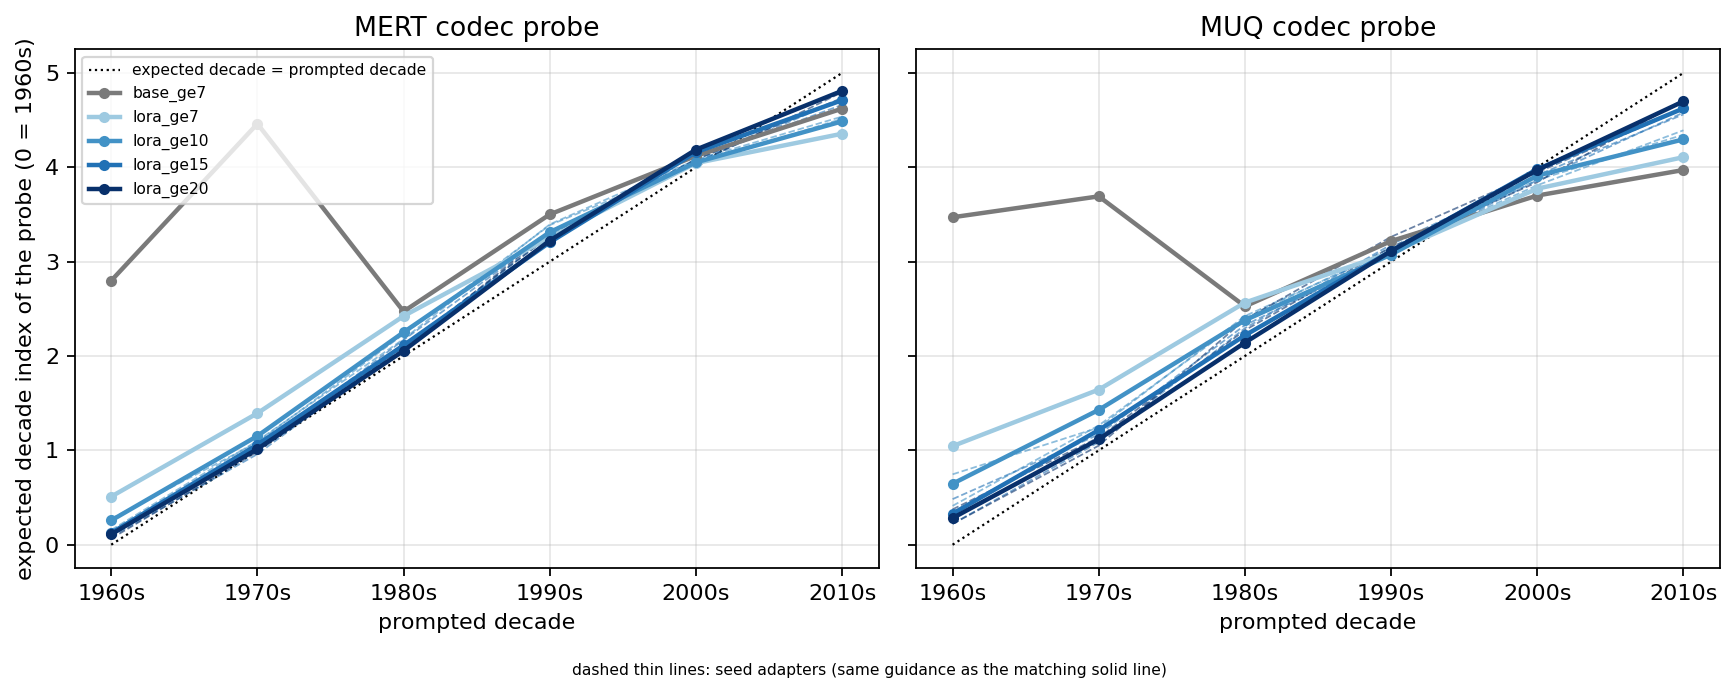
\includegraphics[width=0.85\textwidth]{six_decades_E.png}
\caption{Expected probe decade per prompted decade (11 configurations: base, LoRA at $g_e\in\{7,10,15,20\}$, and seed adapters as thin dashed lines).}\label{fig:E}
\end{figure*}

\textbf{Six decades.} Table~\ref{tab:six} and Fig.~\ref{fig:E} extend the prompts to the 1970s, 1990s and 2000s. With the adapter, $E$ increases monotonically with the prompted decade in both encoders and in the independent EffNet probe, and every $\dP$ interval excludes 0 in all configurations. The base model does not: its 1970s prompt gives $E{=}4.46$ and a negative $\dP$ ($-.036$, interval excludes 0). The 1990s prompt is the weakest (MERT top-1 target share $.46$ at $g_e{=}10$, $.58$ at 15 and 20). For the 2000s prompt the primary adapter's $\dP$ falls from $+.257$ ($g_e{=}10$) to $+.181$ (20) while $E$ drifts toward the 2010s ($4.05\to4.19$); the two seed adapters do not show this ($+.335$/$+.362$ at 10, $+.377$/$+.347$ at 20), and a pop-punk wording of the 2000s prompt keeps its effect from $g_e{=}10$ to 15 (MERT $+.240$ at both), so the decline is specific to an adapter and a wording. Wording matters strongly for the 1990s: a grunge wording gives MERT $\dP{=}+.098$ and $E{=}3.86$, a eurodance wording $+.413$ at $g_e{=}15$, and no wording beats the default prompt in both encoders.

\textbf{Content and quality.} Song-identification top-1 stays $.84$--$.88$ for the main decades at $g_e{=}7$--20 ($.944$ neutral), chord agreement $.33$--$.36$ (rotation floor $.02$). For the extra decades it falls with $g_e$ (1970s $.833$ at 10, $.764$ at 20) and chord agreement drops to $.317$--$.337$. Audiobox production quality does not drop (3-branch: $7.50$--$7.52$ vs.\ $7.31$ neutral); the 2000s prompt loses $0.27$ PQ only at $g_e{=}20$. KAD-style margins rise with $g_e$ (same encoder family as the probe, so not independent). FD-VGG against real clips of the prompted decade is lower than neutral for the 1980s and 2010s in both seed adapters at $g_e{=}7$ and $10$ (interval excludes 0 in 7 of 8 cells; 2010s: $-1.9$ to $-2.1$) but not for the 1960s; for $g_e\geq15$ the 2010s gain stays significant and the 1980s gain no longer is, and 72 clips per cell keep intervals wide ($\approx\pm1$). For the seed adapters at every guidance level and all six decades, the mean KL-PaSST to the original clip is lower than neutral ($-0.18$ to $-0.42$) and the mean CLAP text score higher ($+.04$ to $+.26$), i.e.\ era-prompted clips remain classified like their originals (not so for every base-model cell, e.g.\ 2010s KL $+.025$). We therefore recommend $g_e{=}7$--10, where the probes, FD, quality and identity agree (interpretation).

\textbf{Other generators.} MuseControlLite (Stable Audio Open with melody adapter) preserves the melody more strictly (top-1 $1.000$) but the same prompts barely move the probes (MERT 2010s $+.171$, others $\leq +.015$); ACE-Step 1.5 in cover mode moves the 1960s and 1980s probes ($+.05$--$+.08$, $+.13$--$+.22$ in MERT) but keeps much less of the song (top-1 $.27$--$.35$ at every strength). Text-only MusicGen keeps $.188$ song-identification, showing that the chroma condition, not the kept vocal, preserves identity.

\section{What else moves the probes}
\textbf{Probe training set.} Training on original stems, codec-resynthesised stems, their union, and double-codec stems gives the same sign and similar size for 1980s and 2010s (differences $\leq.09$ for double-codec); a probe trained only on original stems barely registers the generated 1980s (MERT $+.01$ to $+.23$ vs.\ $+.25$ to $+.83$ codec-matched), which is why we use codec-matched probes.

\textbf{Bandwidth.} Band-limiting the real accompaniment moves the probes toward earlier decades (MuQ $-.61$, MERT $-.30$ expected decades) and so does added hiss; soft clipping, limiting and a high shelf do not. Era prompts change high-frequency content in every system ($+4$ to $+12$\,dB above 7\,kHz for the 1980s prompt), with weak-to-moderate correlation between spectral change and probe change (Spearman up to $.44$). Matching each era clip's long-term spectrum to its neutral clip leaves MERT 1980s and 2010s effects positive (three-branch $g_e{=}10$: $+.648\to+.553$, $+.424\to+.406$) and the 1960s effect unchanged; the MuQ 2010s effect halves ($+.370\to+.187$) and the base-model MuQ 2010s effect disappears ($+.094\to-.044$, interval includes 0). Finally, prompts that name no decade but only bandwidth change the expected decade of the same generator: ``dull, band-limited, tape hiss'' shifts it by $-1.34$ (MERT) and $-0.98$ (MuQ) at $g_e{=}10$ (the 1960s prompt shifts it by $-2.79$ and $-2.29$), and ``bright, full-bandwidth'' by $+0.42$ and $+0.97$. Part of the era effect is thus carried by bandwidth; the spectrum-matching control shows it is not all of it. A hard decoder-level bandwidth constraint was not run.

\textbf{Nuisance removal.} We fit a LEACE eraser on the training embeddings of codec-resynthesised accompaniment for two nuisance concepts, ten principal components of Discogs-EffNet style tags of the original mix (genre proxy) and nine signal statistics of the accompaniment stem (bandwidth and noise-floor proxy), retrain the era probe on the erased features, and apply the same eraser to the generated clips. Table~\ref{tab:nuis} shows that every adapter-plus-guidance effect stays positive with intervals excluding 0 in both encoders, at $g_e{=}7,10,20$ and for both seed adapters, but shrinks by $.07$ to $.27$; a random projection of the same rank changes nothing (within $.004$). The base model's 2010s effect disappears (MERT $+.328\to-.020$, MuQ $+.094\to+.010$) while its 1980s effect does not ($+.593\to+.608$), so the base 2010s effect is carried by these nuisance directions and its 1980s effect is not. The erased probes are weaker on real audio (MuQ accuracy $.432\to.295$), so some shrinkage may reflect a weaker probe, and erasure also moves the neutral reference.

\begin{table}[t]\centering\footnotesize
\setlength{\tabcolsep}{2pt}
\caption{MERT $\dP$ (1960s / 1980s / 2010s) before and after erasing style and bandwidth nuisance directions (rank 19).}\label{tab:nuis}
\resizebox{\columnwidth}{!}{\begin{tabular}{@{}lcc@{}}\toprule
System & No erasure & Erased\\\midrule
Base, std.\ guidance & $-.001$ / $+.593$ / $+.328$ & $+.069$ / $+.608$ / $-.020$\\
LoRA alone & $+.396$ / $+.246$ / $+.171$ & $+.179$ / $+.165$ / $+.050$\\
+3-branch $g_e{=}10$ & $+.698$ / $+.648$ / $+.424$ & $+.489$ / $+.503$ / $+.249$\\
+3-branch $g_e{=}20$ & $+.759$ / $+.826$ / $+.649$ & $+.613$ / $+.747$ / $+.476$\\\bottomrule
\end{tabular}}
\end{table}

\textbf{Evaluator disagreement.} The zero-shot audio-language judge is weak on real clips (exact-decade accuracy near chance, Spearman $.45$--$.67$ with the true decade); it confirms the 1980s effect of the base model but not the adapter's 1980s and 2010s effects. CLAP and the probes agree on the sign of 2010s shifts for guidance variants but disagree for the 1960s of some adapters. We treat the probes as proxies, not as measures of perceived era.

\section{Limitations}
Release decade is not recording era (reissues, Sec.~\ref{sec:data}); we could not recover Discogs ids for our clips, so splits are artist-disjoint but not guaranteed clique-disjoint (covers or reissues of one composition could cross partitions) and no clean original-release subset could be built. 24 validation songs, 3 seeds, one validation split per task whose results also guided choices such as layer and guidance scale, no artist ids (so no artist-grouped intervals; pooled out-of-fold analyses are not artist-disjoint), hidden test labels. Language and genre are proxies (Whisper LID, Discogs-EffNet tags). Probe-based era scores are proxies trained on the same real clips whose labels they predict; each conclusion is reported with at least two encoders and a third family where possible. One generator family carries the main result and the only external baselines are MuseControlLite and ACE-Step, not the stronger controllers above; the melody condition is full-mix chroma; the learned adapter is generic (decade-labelled), and the nuisance-erasure analysis is a diagnostic: the discovered cues are not used to steer generation; a single training recipe has three adapter seeds, and several comparisons are single runs. The wording of the 1990s and 2000s prompts changes results. No listening test has been run, so we make no claim about perceived era or audio quality beyond automatic metrics.

\section{Conclusion}
Release decade is mostly read from the accompaniment and release market from the vocal, largely through sung language (a smaller signal remains for English-sung clips); both are properties of editions, and part of the decade signal travels with genre and recording bandwidth. A melody-preserving cover can be pushed along the decade axis by an adapter plus a melody-preserving era-contrast guidance rule, with probe-measured effects that replicate across adapter seeds and encoders and no measured loss of song identity at moderate guidance, but the effect partly rides on bandwidth cues and is wording-dependent for the 1990s and 2000s.

\paragraph{Reproducibility.} Code, every result file and a worklog with each run's configuration are in \url{https://github.com/goog-msft-fb-nflx-nvda-aapl/music-info-research} (folder \texttt{topics/era\_market\_cover}); \texttt{src/99\_make\_all\_tables.sh} regenerates all tables from stored results and was run from a fresh clone with identical output. Generated audio, embeddings and the source clips are not in the repository.

\bibliographystyle{unsrtnat}
\bibliography{refs}
\end{document}
